

\section{Julia implementation}\label{sec:implementation}

The computer code is implemented in Julia language~\cite{} according to the workflow described below, whose stages are parallelized and/or optimized in various ways.

\subsection{Parallel workflow}\label{sec:implementation}


\paragraph{Workflow setup} The functions in this preliminary step include:
\begin{enumerate}

\item input of 3D medical image $\mathcal{I}$ dimensions $\ell_1, \ell_2, \ell_3$, such that: $\mathcal{I} = [\ell_1]\times[\ell_2]\times[\ell_3]$, where $[\ell_k] = (1,2,\ldots,\ell_k)$;

\item analysis of resources available in the computational environment, including operating system, type and number of compute nodes (processors, cores, GPUs), number of cores per node, RAM and caches amounts;

\item depending on the above, best decision for $\emph{size}$ of 3D image blocks $\mathcal{B}$ (bricks); defaults to: $\emph{size}=64$; hence the number of bricks will be $n=\ceil{\ell_1/size}\times\ceil{\ell_2/size}\times\ceil{\ell_3/size}$. 
Hence default value: $n=256$, for images $\mathcal{I} = 512\times 512\times 256$;

\item computation of a Julia's sparse boundary matrix $[\partial_B]$, returning a value of type \texttt{SparseMatrixCSC\{Int8\}\{Int64\}}, where \texttt{Int8} and \texttt{Int64} are the types for values and indices, respectively, stored by Compressed Sparse Column (CSC) format; the average $[\partial_B]$ (for $\emph{size}$ = 64) is about 45 MB;

\item creation of either a local or distributed channel to implement a producer/consumer model of parallel/distributed computation, depending on available resources;

\item distribution of matrix $[\partial_B]$, of default size $45$ MB, to all available nodes/cores (workers) using the macro \texttt{@eveywhere}. 

\end{enumerate}

<<<<<<< HEAD
The memory occupancy of the sparse matrix is computed by considering $8+1$ bytes for non-zero element (which are exactly 6 per row), plus 8 bytes per each index of column start.  
With $size=64$, the number of non-zeros within the sparse matrix $[\partial_{64^3}]$ is $\mathtt{nnz} = 4 792 266$, for a storage size of $9\times \mathtt{nnz}+8\times 262144 \simeq 45$ MB. 
=======
\begin{figure}[htbp]
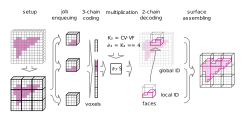
\includegraphics[width=0.99\textwidth]{figs/schema_horizontal.pdf} 
%\includegraphics[scale=1]{input/ircad_comparison.pdf} 
\caption{Workflow of LAR-SURF algorithm}
\label{fig:schema}
\end{figure}

With $size=64$, the number of non-zeros within the sparse matrix $[\partial_{64^3}]$ is $\mathtt{nnz} = 4 792 266$, for a memory size of $9\times \mathtt{nnz}+8\times 262144 \simeq 45$ MB. The memory size of the sparse matrix is computed by considering $8+1$ bytes for non-zero element (which are exactly 6 per row), plus 8 bytes per each index of column start.  

>>>>>>> f5c1ade674505d34a52843fee9697d472b4d29eb

\paragraph{Job enqueuing} Communication and data synchronization may be managed through \emph{Channels}, which are the FIFO conduits that may provide producer/consumer communication. Overall execution time can be improved if other tasks can be run while a task is being executed, or while waiting for an external service/function to complete. The single work items of this stage follow:
\begin{enumerate}

\item extraction, from image arrays of the block views, depending on 3 Cartesian indices;

\item transform  each block \emph{from global} $[\ell_1]\times[\ell_2]\times[\ell_3]$ to \emph{local coordinates} $[n]\times[n]\times[n]$;

\item further transform of each \emph{foreground voxel} $\nu\in\mathcal{S}\subseteq\mathcal{I}$ from Cartesian to linear coordinates, using the suitable Julia's library functions.

\item enqueing the job (as a sequence of integer positions for the non-zeros image elements aligned in a memory buffer of proper \texttt{Channel} type).
\end{enumerate}

\paragraph{3-Chain encoding} 
The interesting part of the \emph{Image} $\mathcal{I}$ is called \emph{Segment} $\mathcal{S}$. The goal of the whole \emph{workflow} is to extract a \emph{boundary model} of $\mathcal{S}$ from $\mathcal{I}$. The portion of $\mathcal{S}$ inside $\mathcal{B}$, will be denoted as $\mathcal{S}(B)$.
Each block $\mathcal{B}$ of the 3D image must by converted into the \emph{coordinate representation} of a vector $\nu\in C_3$ in the linear space  of 3-chains. 

In coordinates local to $\mathcal{B}$, once fixed an ordering from Cartesian to linear coords, this vector is represented by a \emph{binary array} of length $size^3$. With $size=64$, we have $64^3=262144$,  with a non-zero value (i.e.~$1$) for each foreground voxel in $\mathcal{S}(B)$. Therefore, the coded segment portion $\mathcal{S}(B)$, results with a space occupancy of about $262$ KB if encoded as a full array (i.e.~including the zero values). Whether encoded as a sparse vector, its space occupancy will correspondingly decrease.

\begin{enumerate}

\item each encoding task produces either a full or sparse binary vector. With full or sparse arrays depending by one index, we get either 262 KB or less per job, correspondingly;

\item special format for sparse CSC (Compressed Sparse Column) vectors can be used, since the \emph{value} data for non-zeros does not need storage. Hence only a single 1-array of \texttt{Int64} row positions (with total length equal to the number of non-zeros in the block, with $8\times\mathtt{nnz}$ kB storage) is needed;

\item prepare subsequences of such data vectors (non-zero linear row indices), in order to feed efficiently the available processor threads.
In case of presence of one/more GPUs, a smaller size of the block---and hence of the boundary matrix and the encoded 3-chain vectors---and then much higher vector numbers, are preferable for speed.

\end{enumerate}

\paragraph{SpMM Multiplication} 
According to the current literature~\cite{} it is more convenient to execute SpMV (sparse matrix-vector) multiplications than SpMSpV (sparse matrix-sparse vector) multiplications. Since we have 256 such jobs (one multiplication per block) to perform in the standard setting of the algorithm\footnote{
Size of block $64^3$; size of image $512^2\times 256$.
}, or more in case of either smaller blocks or image greater than the standard one, this stage must be evidently parallelized and carefully tuned, possibly by using the GPU, if available.
\begin{enumerate}

\item Various multiplication algorithms are being experimented, using several packages for sparse linear algebra and/or custom implementations;

\item the total speed of this stage will strongly depend on the hardware available, on the granularity of blocks, and on the choice between dense/sparse storage of encoded 3-chains;

\item anyway, the compute elements or threads will be feed without solution of continuity in a \emph{dataflow} process. This parallel operation is, according to our preliminary experiments, the critical one of the whole workflow, in the sense that any $\Delta T$ (either positive or negative) in this stage will contribute to the total time $T$.

\end{enumerate}

\paragraph{2-Chain decoding} 
Each multiplication of $[\partial_B] : C_3 \to C_2$, times a 3-chain $\nu\in C_3$, produces a 2-chain  $\sigma\in C_2$, i.e.~the \emph{coordinate representation} of the \emph{boundary vector} $\sigma\in C_2$.  The inverse of the coding algorithm is executed in the present stage.  This process can also be partially superimposed in time with the previous ones, depending on the size of the memory buffers used to feed the CPU cores or the GPUs and get their results. Some elementary steps follow:

\begin{enumerate}

\item conversion from position of ones (or non-zeros) in the 2-chain to linear indices of rows;

\item conversion from linear indices to Cartesian indices in coordinates local to the $\mathcal{B}$ block, using the appropriate library functions;

\item conversion from each Cartesian index value to a suitably oriented (i.e.~with proper attitude) geometry quadrilateral (or pair of triangles) in local coordinates.

\end{enumerate}

A Julia's vectorized pipeline dataflow seems the more appropriate implementation model for the job of each worker.

\paragraph{Assembling and artifact filtering} 
The results of the previous stages can be described as a \emph{collection of sets} of \emph{geometric quadrilaterals (quads)}, each one encoded as an array of quadruples of integer indices, pointing to the linear array of grid vertices associated to the image block $\mathcal{B}$.  In other words, \emph{all quads} of \textbf{each job} are now given in the \textbf{same} \emph{local coordinates}.  Besides to put each partial surface $\mathcal{S}(B) = (\texttt{V}_B, \texttt{FV}_\sigma)$ in the global coordinate system of the image, the present stage must eliminate the redundant boundary features possibly generated at the edges of the partial surface $\mathcal{S}(B)$ within each block $\mathcal{B}$ such that $B \cap \mathcal{I} \not= \emptyset$:
\begin{enumerate}

\item translate each array $\mathtt{FV}_\sigma$, of type \texttt{Lar.Cells}, by summing to each vertex index the linearized offset of the Cartesian coordinates $(n,m,p)(B)$ of the $\mathcal{B}$'s \emph{reference vertex}, i.e.~the one with (all) lowest \emph{Cartesian coordinates} within the $\mathcal{B}$ block.

\item remove both instances of \emph{double quads} generated by \texttt{Lar} software at the block boundaries (see Figure~\ref{fig:blockboundary}). They are artifacts generated by the decomposition of the whole image into a number of blocks of tractable size.

\item 
a smart strategy of removal of such artifacts may be used, which does not require any sorting nor searching on the assembled array of quads. It will consist in arranging each block with all three dimensions decreased-increased by one, so that each 2-adjacent pair of blocks will be covering each other for a full side extent of blocks of depth one. The details of this \emph{artifact filtering} are elucidated in Section~\ref{sec:covering}.

\end{enumerate}

\paragraph{Smoothing} 
The final smoothing of the generated surfaces cannot be performed block-wise, since this would introduce smoothing artifacts at the block boundaries. Anyway, the Taubin smoothing~\cite{} can be performed in parallel, since for each vertex in the final surface (except eventually the ones on the image $\mathcal{I}$ boundaries) it essentially consist in computing a new position as a proper average of its neighborhood vertices, i.e.~by applying a discrete Laplacian operator.  Some appropriate set workers may so be assigne the task of generating iteratively a new position for the vertices they take cure of. In particular, we have:
\begin{enumerate}

\item Job enqueuing, by writing sets of integers (global linear indices of vertices) in array buffers of appropriate type \texttt{Channel};

\item iterated vectorized computation of proper averages of closed vertices;

\item job dequeuing, by recovering finished tasks from a channel and assembling the results into the embedding function $\mathtt{V}: C_0 \to \E^3$ providing an array of type \texttt{Lar.Points} of \texttt{Float64 $\times$ 3}, with vertex coordinates by column.
\end{enumerate}



\subsection{Performance analysis}\label{sec:analysis}

The size of boundary matrix is critical parameter of LAR-SURF method. To determine optimal size of boundary matrix the experiment on artifical data was performed (Fig.  \ref{fig:bm_size_tesla}). Size of experimental data is set to $512\times512\times512$ and it is derived from typical size of Computed Tomography medical images. Computation is done on Tesla DGX-1 machine.

\begin{figure}
\centering
\includegraphics[width=0.6\textwidth]{figs/bm_size_tesla.pdf} 
%\includegraphics[scale=1]{input/ircad_comparison.pdf} 
\caption{Time requirements of LAR-SURF filter used on artificial with different size of boundary matrix}
\label{fig:bm_size_tesla}
\end{figure}



To compare time requirements of LAR-SURF with Marching Cubes implemented in Python we performed experiment on Ircadb dataset \cite{ircad}. Dataset contain 20 Computed Tomography images (see table \ref{tab:ircad1}) with xy-resolution from 0.56 mm to 0.87 mm and z-resolution from 1.0 mm to 4.0 mm. The number of slices is each series varies from 74 to 260 and size of each slice is $512\times512$. Dataset contain manually segmented liver, portal vein and other structures. We performed surface extraction of liver with Marching Cubes and LAR-SURF. Time required for computation can be seen on figure \ref{fig:ircad_comparison}. 

Based on t-test with $\alpha=0.99$, $p=\num[]{8.735e-24}$ and 
$s=\num[]{-16.67}$ it can be shown that the mean of time consumed by LAR-SURF is significantly lower from time consumed by Marching Cubes.


\begin{figure}
\centering
\includegraphics[width=0.99\textwidth]{figs/ircad_comparison.pdf} 
%\includegraphics[scale=1]{input/ircad_comparison.pdf} 
\caption{Time requirements of LAR-SURF filter and Marching Cubes on Ircad dataset. Error bars shows the 95\% confidence interval}
\label{fig:ircad_comparison}
\end{figure}



